\begin{figure}[h]
	\begin{center}
  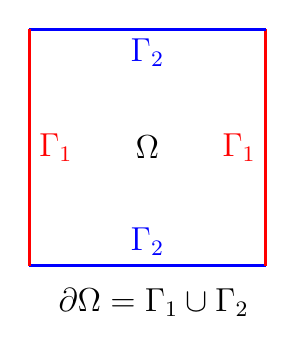
\begin{tikzpicture}[scale=0.5]
    \tikzstyle{every node}=[font=\tiny]
    \draw[style=very thick,color=blue] (0,0)
    node[fill=none, below right=1ex, color=black] { { \large $\partial\Omega = \Gamma_1 \cup \Gamma_2$ } }
    -- (3,0) -- (6,0);
    \draw[style=very thick,color=red] (6,0) -- (6,3) -- (6,6);
    \draw[style=very thick,color=blue] (6,6) -- (3,6) -- (0,6);
    \draw[style=very thick,color=red] (0,6) -- (0,3) -- (0,0);

    \draw (3,3) node[fill=none] { {\large $\Omega$} };
    \draw[color=red] (0,3) node[fill=none,right] { {\large $\Gamma_1$} };
    \draw[color=blue] (3,0) node[fill=none,above] { {\large $\Gamma_2$} };
    \draw[color=red] (6,3) node[fill=none,left] { {\large $\Gamma_1$} };
    \draw[color=blue] (3,6) node[fill=none,below] { {\large $\Gamma_2$} };
  \end{tikzpicture}
	\end{center}
  \caption{Decomposed Boundary}
	\label{fig:SplitBoundary}
\end{figure}
